\usepackage{graphicx}\newpage
\thispagestyle{fancy}
\vspace{\fill}
\subsection{Tela de comando Alimentação}
Esta tela é acessada pelo botão "\textgreater" no menu superior esquerdo da tela de comando de máquina, pelo botão "\textless{}" no menu superior esquerdo da tela comando impressoras ou impressora 1, pelo botão "ALM" em qualquer tela de comando e pelo botão comando da tela ajustes alimentação. A partir desta os botões "comando" e "ajustes" começam a se comportar de maneira contextual de maneira que eles vão levar a tela correspondente a tela selecionada. Caso você já esteja na tela selecionada você será levado a tela anterior.

\begin{figure}
    \centering
    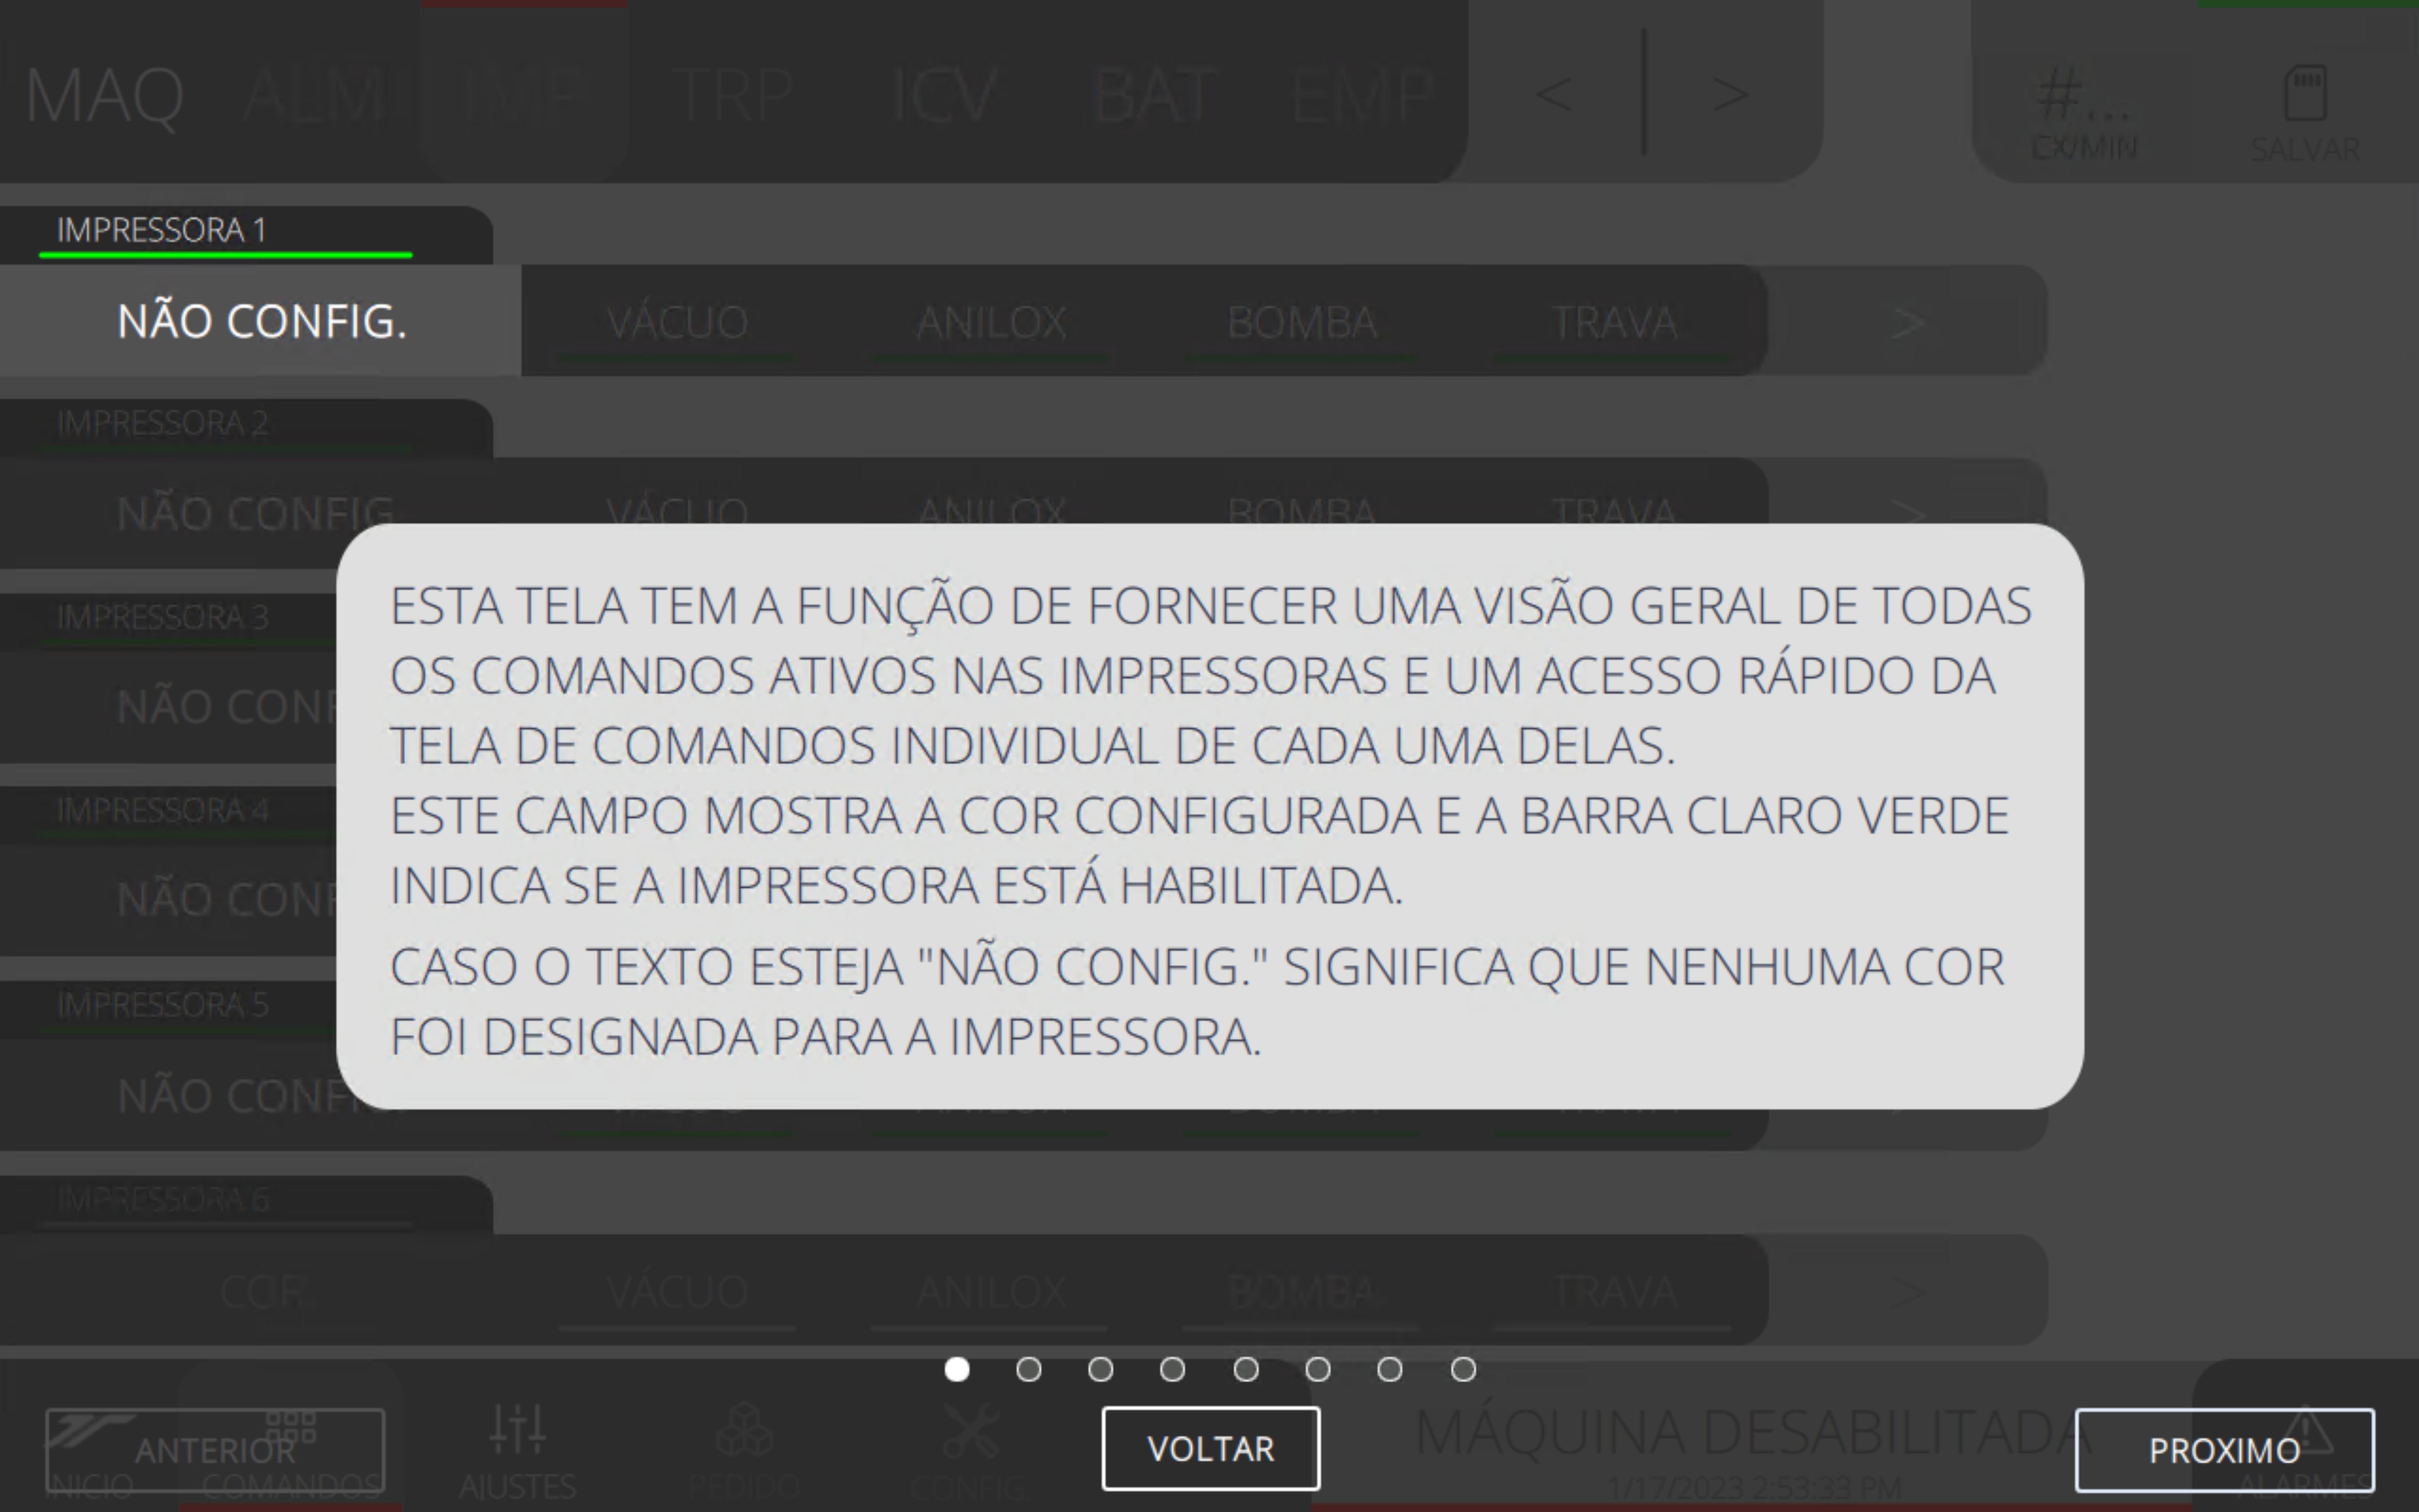
\includegraphics[width=480,height=300]{imagesICV/03-feeder/commands/1}
    \caption{Tela de comando Alimentação}
    \label{fig:}
\end{figure}